\documentclass{mipt-thesis-bs}
% Следующие две строки нужны только для biblatex. Для inline-библиографии их следует убрать.
\usepackage{mipt-thesis-biblatex}
\usepackage[justification=centering]{caption}
\usepackage{glossaries}
\usepackage{url}
\usepackage{pdfpages}
\usepackage{hyperref} 
\addbibresource{ref.bib}


\title{Применение генеративного моделирования как инструмента постановки естественнонаучной задачи педагогической направленности}
\author{Машалов Никита}
\supervisor{Щербаков Дмитрий}
%\referee{Петров Д.\,Е.}       % требуется только для mipt-thesis-ms
\groupnum{БО2-886}
\faculty{Физтех-школа физики и исследований им. Ландау}
\department{Кафедра инновационной педагогики}


\begin{document}
% Абстракт
\chapter{Введение}

Педагогическая задача является основой образовательного процесса и играет ключевую роль в достижении учебных целей. Её цель состоит в том, чтобы обеспечить студентам определённые образовательные возможности и помочь им развить необходимые знания, умения и навыки.

При создании педагогической задачи важно учитывать не только содержание обучения, но и индивидуальные особенности студентов, их уровень знаний и способности. Педагогическая задача должна быть четко сформулирована, чтобы студенты могли понять, что от них требуется, и чувствовать уверенность в выполнении задания.

Важным аспектом педагогической задачи является её реалистичность и актуальность. Задача должна иметь практическую ценность и быть связанной с реальными жизненными ситуациями или профессиональными задачами. Это поможет стимулировать интерес и мотивацию студентов к изучению материала.

Педагогическая задача также должна предоставлять возможность для развития критического мышления и применения знаний на практике. Она должна быть структурированной и обеспечивать возможность оценки выполнения студентами поставленной задачи. Критерии оценки должны быть ясными и объективными, чтобы обеспечить справедливую оценку достижения учебных целей.

Реализация педагогической задачи может включать использование различных методов обучения и оценки, таких как групповая работа, проектная деятельность, обсуждения, решение проблемных ситуаций и другие. Это позволит стимулировать активное участие студентов в образовательном процессе и способствовать их полноценному развитию.


В академическом контексте условие задачи должно быть представлено в понятной и ясной формулировке, чтобы студенты могли полностью понять, что от них требуется. Это важно для обеспечения эффективного обучения и достижения учебных целей. При этом условие задачи должно быть достаточно простым, чтобы студенты могли легко освоить материал и выполнить задание, но при этом содержательным, чтобы оно имело академическую ценность и было связано с обучающей программой других предметов.

Параллели с обучающей программой других предметов могут быть важны для того, чтобы показать студентам связь между различными областями знаний и помочь им понять, как полученные знания применяются на практике. Например, задача по математике может быть сформулирована таким образом, чтобы студенты могли увидеть её применение в других предметах, таких как физика или экономика.

Кроме того, условие задачи должно быть структурированным и логически последовательным, чтобы студенты могли легко следовать указаниям и выполнять задание без лишних затруднений. Это позволит им сконцентрироваться на освоении материала и достижении желаемых результатов.

Таким образом, условие задачи должно быть простым и понятным, иметь параллели с обучающей программой других предметов и быть структурированным и логически последовательным, чтобы обеспечить эффективное обучение и достижение учебных целей.

\chapter{Методика составления педагогических задач}
В рамках секции будут описаны методы, применяемые в генеративном моделировании
для решения задачи генерации задач.


\begin{figure}[h]
    \centering
    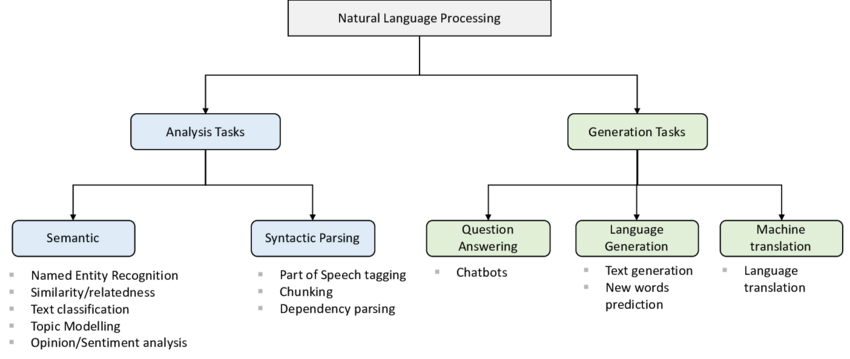
\includegraphics[width=0.5\textwidth]{assets/llm/taxonomy.png}
    \caption{Таксономия современных подходов обработки естественного языка}
    \label{llm_taxonomy}
\end{figure}




\section{Использование нейросетевых подходов}

В рамках раздела будет последовательно изложена хронология подходов
для построения генеративных моделей языка.

 модели строились на n-граммах
 


В последствии подходы развивились примением реккурентных нейронных сетей LSTM \cite{HochSchm97} и GRU



С эффективным примением архитектуры нейронной сети Attention \cite{NIPS2017_3f5ee243}, позволяющей эффективно обучать нейронные сети на графических ускорителях. 




\section{Обработка естественного языка}

\subsection{Методы обработки естественного языка}

Анализ естественного языка это межпредметная дисциплина.
Компьютерная лингвистика

Практически востребованной оказалась дистрибутивная гипотеза \cite{Schutze},
легшая в основу алгоритма \cite{NIPS2013_9aa42b31}


**Лемматизация** - процесс приведения языка к нормальной форме.

**


\section{Обработка изображений}



\chapter{Методы машинного обучения для работы с текстом и изображениями}
В рамках секции будут описаны методы, применяемые в генеративном моделировании
для решения задачи генерации задач.


\begin{figure}[h]
    \centering
    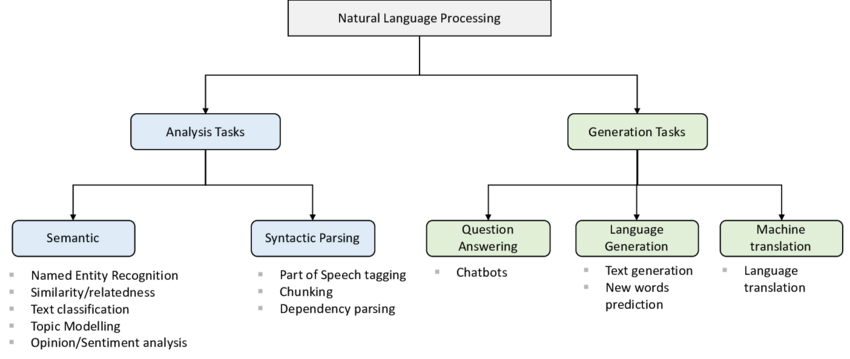
\includegraphics[width=0.5\textwidth]{assets/llm/taxonomy.png}
    \caption{Таксономия современных подходов обработки естественного языка}
    \label{llm_taxonomy}
\end{figure}




\section{Использование нейросетевых подходов}

В рамках раздела будет последовательно изложена хронология подходов
для построения генеративных моделей языка.

 модели строились на n-граммах
 


В последствии подходы развивились примением реккурентных нейронных сетей LSTM \cite{HochSchm97} и GRU



С эффективным примением архитектуры нейронной сети Attention \cite{NIPS2017_3f5ee243}, позволяющей эффективно обучать нейронные сети на графических ускорителях. 




\section{Обработка естественного языка}

\subsection{Методы обработки естественного языка}

Анализ естественного языка это межпредметная дисциплина.
Компьютерная лингвистика

Практически востребованной оказалась дистрибутивная гипотеза \cite{Schutze},
легшая в основу алгоритма \cite{NIPS2013_9aa42b31}


**Лемматизация** - процесс приведения языка к нормальной форме.

**


\section{Обработка изображений}



\chapter{Описание работы}
В рамках секции будут описаны методы, применяемые в генеративном моделировании
для решения задачи генерации задач.


\begin{figure}[h]
    \centering
    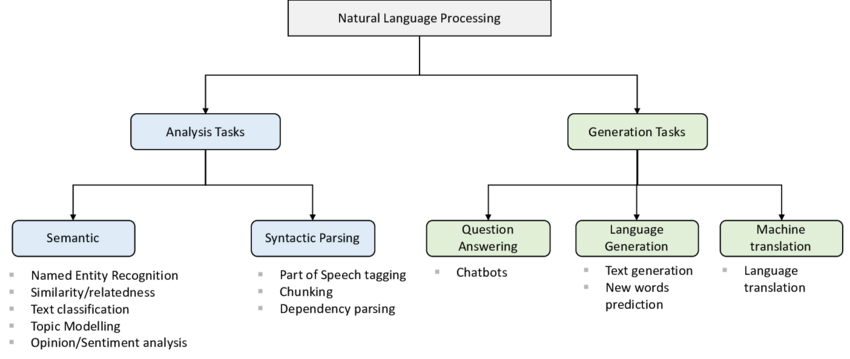
\includegraphics[width=0.5\textwidth]{assets/llm/taxonomy.png}
    \caption{Таксономия современных подходов обработки естественного языка}
    \label{llm_taxonomy}
\end{figure}




\section{Использование нейросетевых подходов}

В рамках раздела будет последовательно изложена хронология подходов
для построения генеративных моделей языка.

 модели строились на n-граммах
 


В последствии подходы развивились примением реккурентных нейронных сетей LSTM \cite{HochSchm97} и GRU



С эффективным примением архитектуры нейронной сети Attention \cite{NIPS2017_3f5ee243}, позволяющей эффективно обучать нейронные сети на графических ускорителях. 




\section{Обработка естественного языка}

\subsection{Методы обработки естественного языка}

Анализ естественного языка это межпредметная дисциплина.
Компьютерная лингвистика

Практически востребованной оказалась дистрибутивная гипотеза \cite{Schutze},
легшая в основу алгоритма \cite{NIPS2013_9aa42b31}


**Лемматизация** - процесс приведения языка к нормальной форме.

**


\section{Обработка изображений}



\chapter{Заключение}
\

\section{Благодарности}

Автор благодарит кафедру инновационной педагогики за предоставление консультационной инфоромации в области права
и . Отдельная благодарность моему научному руководителю Щербакову Дмитрию Евгеньвичу
за возможность работы в актуальной и современной тематики генеративного моделирования

\printbib

\end{document}